\section{Introduction}
Das ist der Einleitungsteil unserer Hausarbeit, die bei weitem noch nicht fertig ist.

\subsection{Research question}
Kleiner Reminder für mich in Bezug auf die Dinge, die wir bei der Thesis beachten sollten und \LaTeX{}-Vorlage für die Thesis.

\subsection{Research objective}
chapter \ref{infos} enthält die Inhalte des Thesis-Days und alles, was zum inhaltlichen erstellen der Thesis relevant sein könnte. In chapter \ref{latexDetails} \nameref{latexDetails} findet ihr wichtige Anmerkungen zu \LaTeX{}, wobei die wirklich wichtigen Dinge im Quelltext dieses Dokumentes stehen (siehe auch die Verzeichnisstruktur in Abbildung \ref{fig:verzeichnisStruktur}).

\subsection{Motivation for researching WASM}

\begin{figure}[H]
\caption{Verzeichnisstruktur der \LaTeX{}-Datein}\label{fig:verzeichnisStruktur}
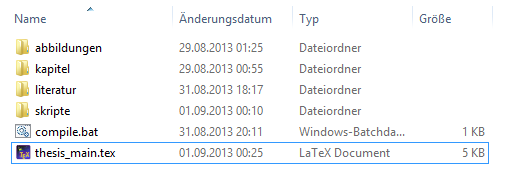
\includegraphics[width=0.9\textwidth]{verzeichnisStruktur}
\\
Quelle: Eigene Darstellung
\end{figure}
